\documentclass[12pt,a4paper]{article}
\usepackage[utf8]{inputenc}
\usepackage[T1]{fontenc}
\usepackage[portuguese]{babel}
\usepackage{geometry}
\usepackage{graphicx}
\usepackage{longtable}
\usepackage{booktabs}
\usepackage{array}
\usepackage{enumitem}
\usepackage{xcolor}
\usepackage{hyperref}
\geometry{margin=2.5cm}
\setlength{\parindent}{0pt}
\setlength{\parskip}{0.65em}
\setlist[itemize]{leftmargin=*, topsep=0.2em}
\hypersetup{colorlinks=true, linkcolor=blue, urlcolor=blue}
\graphicspath{{images/}}
\sloppy

\begin{document}

\begin{titlepage}
\centering
\vspace*{2cm}
{\Huge\bfseries ANCIENTCOINS\par}
\vspace{0.6cm}
{\Large Aplicação para Gestão de Coleções Numismáticas\par}
\vspace{0.35cm}
{\large Relatório de Projeto - Interação Homem-Máquina\par}
\vfill
{\large\bfseries Autores Grupo 43\par}
Rui Mendonça -- 29738 (ruimendonca@ipvc.pt)\par
Cristiano Fonseca -- 29725 (c.fonseca@ipvc.pt)\par
Gonçalo Sousa -- 29726 (goncalosousa@ipvc.pt)\par
\vfill
Interação Homem-Máquina\par
Ano Letivo 2025/2026\par
\end{titlepage}

\tableofcontents
\newpage

\section*{Resumo}
\addcontentsline{toc}{section}{Resumo}

O presente projeto consiste no desenvolvimento da aplicação móvel AncientCoins, uma plataforma destinada a colecionadores de moedas que pretende facilitar a gestão de coleções pessoais, a compra e venda de moedas e a realização de trocas entre utilizadores. O projeto foi desenvolvido no âmbito da unidade curricular de Interação Homem-Máquina, aplicando metodologias de análise de utilizadores, modelação conceptual, prototipagem, desenvolvimento iterativo e avaliação heurística.

A aplicação foi desenvolvida utilizando Ionic Framework, Angular e Supabase, permitindo a criação de uma solução moderna, responsiva e preparada para utilização em dispositivos móveis. Durante o desenvolvimento foram implementadas funcionalidades de autenticação, gestão de coleção, mercado de compra e venda, sistema de mensagens e perfis de utilizador.

O resultado corresponde a uma aplicação funcional que responde aos requisitos identificados na fase inicial do projeto, proporcionando uma experiência de utilização consistente, intuitiva e alinhada com os princípios estudados na unidade curricular.

\section{Introdução}

\subsection{Enquadramento}

O colecionismo de moedas é uma atividade amplamente difundida entre entusiastas e especialistas da área da numismática. Apesar da existência de diversas plataformas dedicadas à compra e venda de moedas, muitas delas apresentam limitações relativamente à gestão integrada das coleções pessoais e à interação entre colecionadores.

Com o crescimento da utilização de dispositivos móveis, tornou-se pertinente desenvolver uma aplicação que permitisse reunir num único ambiente as principais necessidades dos colecionadores, incluindo catalogação de moedas, gestão de coleções, comunicação entre utilizadores e realização de transações.

Neste contexto surgiu o AncientCoins, uma aplicação móvel concebida para facilitar a gestão de coleções numismáticas e promover a interação entre colecionadores através de um mercado integrado.

\subsection{Objetivos}

O principal objetivo do projeto consiste no desenvolvimento de uma aplicação móvel para colecionadores de moedas. Como objetivos específicos definiram-se:

\begin{itemize}
\setlength{\itemsep}{0.15em}
\item Permitir o registo e autenticação de utilizadores;
\item Gerir coleções pessoais de moedas;
\item Publicar moedas para venda ou troca;
\item Pesquisar moedas disponíveis no mercado;
\item Estabelecer comunicação entre compradores e vendedores;
\item Consultar perfis de utilizadores;
\item Implementar um sistema de avaliações;
\item Garantir uma experiência de utilização intuitiva e consistente.
\end{itemize}

\section{Análise de Tarefas}

A fase inicial do projeto incluiu a realização de um questionário destinado a potenciais utilizadores da aplicação, com o objetivo de identificar as suas necessidades, hábitos de colecionismo e expectativas relativamente a uma plataforma digital de gestão numismática.

O questionário foi respondido por 58 participantes, com idades e perfis diversificados, permitindo recolher dados representativos sobre o público-alvo da aplicação AncientCoins.

\subsection{Análise dos Questionários}

\subsubsection{Perfil dos Respondentes}

\begin{itemize}
\setlength{\itemsep}{0.15em}
\item Sexo: maioritariamente masculino (aproximadamente 75\%);
\item Faixa etária predominante: 18-24 anos (aproximadamente 40\%), seguida de 45-54 anos;
\item Escolaridade variada: desde Ensino Básico até Doutoramento; destaque para Ensino Secundário e Licenciatura;
\item Relação com o colecionismo: cerca de 40\% são colecionadores ativos, 25\% tem interesse, mas ainda não colecionam, 20\% já colecionaram, mas pararam, 15\% sem interesse;
\item Tipos de moedas preferidos: antigas/medievais, comemorativas, nacionais raras;
\item Experiência: de menos de 1 ano a mais de 10 anos de colecionismo.
\end{itemize}

\subsubsection{Ferramentas Atuais de Gestão}

\begin{itemize}
\setlength{\itemsep}{0.15em}
\item Fotografias no telemóvel - método mais comum;
\item Folhas de cálculo (Excel/Sheets);
\item Caderno ou papel;
\item Aplicações específicas (Numista, PCGS CoinFacts, CoinManage, OuoNuma) - uso minoritário;
\item Uma fração significativa não faz qualquer registo.
\end{itemize}

\subsubsection{Canais de Aquisição e Pesquisa}

\begin{itemize}
\setlength{\itemsep}{0.15em}
\item Sites especializados: eBay, Catawiki;
\item Feiras e mercados de colecionismo;
\item Lojas físicas;
\item Grupos em redes sociais;
\item Amigos ou familiares.
\end{itemize}

\subsubsection{Funcionalidades Mais Desejadas}

As funcionalidades mais selecionadas pelos respondentes foram:

\begin{itemize}
\setlength{\itemsep}{0.15em}
\item Registar e catalogar a coleção (escolhida por aproximadamente 80\% dos respondentes);
\item Ver moedas disponíveis de outros utilizadores;
\item Publicar moedas para troca ou venda;
\item Comunicar com outros colecionadores;
\item Receber notificações de moedas de interesse;
\item Tirar fotos diretamente pela app;
\item Ver o valor de mercado das moedas
\end{itemize}

\subsubsection{Dispositivos e Contexto de Uso}

\begin{itemize}
\setlength{\itemsep}{0.15em}
\item Dispositivo preferido: smartphone/telemóvel (aproximadamente 65\% dos respondentes);
\item Computador também relevante (aproximadamente 35\%);
\item Contextos de uso: em casa, em feiras e eventos, em qualquer lugar (uso mobile);
\item Tablet: uso minoritário, mas presente, especialmente em utilizadores mais velhos.
\end{itemize}

\subsubsection{Confiança e Segurança nas Transações}

Dos respondentes que já negociaram, os problemas mais frequentes foram:

\begin{itemize}
\setlength{\itemsep}{0.15em}
\item Moeda diferente do descrito;
\item Suspeita de fraude;
\item Dificuldade de comunicação;
\item Preço injusto;
\end{itemize}

Os fatores de confiança mais valorizados:

\begin{itemize}
\setlength{\itemsep}{0.15em}
\item Avaliações de outros utilizadores;
\item Verificação de identidade dos utilizadores;
\item Fotos detalhadas das moedas;
\item Histórico de transações visível;
\item Moderação da plataforma.
\end{itemize}

\subsection{Questionários da Análise de Tarefas}

Q1 - Quem vai utilizar o sistema?

Com base nos dados do questionário, identificam-se três perfis principais de utilizadores:

Colecionador Ativo Faixa etária: 25-64 anos.

Coleciona há vários anos (1 a 10 ou mais anos). Gere a coleção com Excel ou aplicações específicas. Frequenta feiras e mercados. Já negociou moedas. Utiliza o computador e o telemóvel.

Entusiasta e Principiante Faixa etária: 18-34 anos.

Tem interesse na numismática, mas ainda não coleciona ativamente, ou começou há pouco tempo. Usa principalmente o telemóvel. Nunca negociou. Familiarizado com apps móveis.

Utilizador Casual ou Sénior Faixa etária: 45-65 ou mais anos.

Já colecionou, mas parou, ou tem interesse pontual. Prefere computador ou tablet. Menor familiaridade com apps. Valoriza simplicidade e segurança. Necessita de tutoriais ou ajuda contextual.

Q2 - Que tarefas executa atualmente?

Os utilizadores executam atualmente as seguintes tarefas de forma manual ou dispersa:

\begin{itemize}
\setlength{\itemsep}{0.15em}
\item Fotografam as suas moedas com o telemóvel para registo pessoal;
\item Registam a coleção em folhas de cálculo (Excel) ou cadernos de papel;
\item Pesquisam preços e informações em sites como eBay, Catawiki ou Numista;
\item Compram e vendem em sites generalistas ou grupos de redes sociais;
\item Comunicam com outros colecionadores via redes sociais ou em feiras;
\item Identificam moedas desconhecidas através de pesquisa manual na internet.
\end{itemize}

Q3 - Que tarefas são desejáveis?

Com base nas respostas ao questionário, as tarefas desejadas na aplicação AncientCoins são:

\begin{itemize}
\setlength{\itemsep}{0.15em}
\item Registar e catalogar moedas com fotos, descrição, estado de conservação e valor estimado;
\item Publicar moedas para troca ou venda diretamente na plataforma;
\item Pesquisar e visualizar moedas disponíveis de outros utilizadores;
\item Receber notificações quando aparecem moedas de interesse;
\item Comunicar com outros colecionadores de forma segura dentro da app;
\item Ver o valor de mercado atualizado das moedas;
\item Tirar fotos diretamente pela app para adicionar a coleção;
\item Avaliar e ser avaliado após transações;
\item Consultar histórico de transações e reputação de vendedores.
\end{itemize}

Q4 - Como se aprendem as tarefas?

\begin{itemize}
\setlength{\itemsep}{0.15em}
\item Introdução interativa: tour guiado na primeira utilização, apresentando as funcionalidades principais;
\item Ajuda contextual: ícones de informação junto a funcionalidades menos óbvias;
\item Exploração intuitiva: interface familiar, semelhante a apps como OLX ou Instagram;
\item Suporte via FAQ e guia de utilizador online;
\item Para utilizadores menos experientes: linguagem simples, botões grandes e fluxos lineares.
\end{itemize}

Q5 - Onde são desempenhadas as tarefas?

Versão Web

Em casa, num ambiente controlado. Sessões longas de catalogação e pesquisa detalhada. Ambiente silencioso, boa iluminação, sem pressão de tempo.

Versão Mobile

Em mobilidade: em feiras, em qualquer lugar. Sessões curtas: fotografar, verificar preço, enviar mensagem. Ambiente ruidoso, luz variável, mãos por vezes ocupadas.

Implicação de design

A versão Mobile deve priorizar ações rápidas, botões grandes e feedback imediato. A versão Web pode oferecer funcionalidades mais ricas e formulários detalhados.

Q6 - Quais as relações entre utilizadores e informação?

\begin{itemize}
\setlength{\itemsep}{0.15em}
\item Cada utilizador possui um perfil pessoal com a sua coleção, reputação e histórico de transações;
\item A coleção é privada por defeito, mas pode ser tornada pública;
\item As moedas publicadas para venda ou troca são visíveis por todos os utilizadores registados;
\item As avaliações e histórico de transações são públicos e associados ao perfil do utilizador;
\item Os dados da coleção são sincronizados entre dispositivos (Web e Mobile);
\item Acesso restrito a dados pessoais: só o próprio utilizador pode editar o seu perfil e coleção;
\item Mensagens privadas entre utilizadores: visíveis apenas pelos intervenientes.
\end{itemize}

Q7 - Que outras ferramentas tem o utilizador?

\begin{itemize}
\setlength{\itemsep}{0.15em}
\item Excel e Google Sheets: para registo da coleção (uso muito frequente);
\item Câmara do telemóvel: para fotografar moedas;
\item Numista: catálogo online de moedas (utilizado por vários respondentes);
\item PCGS CoinFacts, CoinManage, OuoNuma: aplicações de nicho já usadas por alguns;
\item eBay e Catawiki: plataformas de compra e venda;
\item Redes sociais (Facebook, grupos de WhatsApp): para comunicação e negociação.
\end{itemize}

A AncientCoins deve posicionar-se como substituto ou complemento destas ferramentas, idealmente permitindo importar dados de Excel e integrar referências do Numista.

Q8 - Como comunicam os utilizadores entre si?

\begin{itemize}
\setlength{\itemsep}{0.15em}
\item Atualmente: grupos de Facebook, WhatsApp, contacto direto em feiras;
\item Na app AncientCoins: comunicação via mensagens privadas integradas;
\item A plataforma facilita a negociação direta entre comprador e vendedor, com proposta de preço ou troca;
\item Sistema de avaliações públicas após cada transação, base para a reputação do utilizador;
\item Notificações push (Mobile) e via e-mail (Web) para novas mensagens ou propostas;
\end{itemize}

Q9 - Qual a frequência de desempenho das tarefas?

Com base nas respostas ao questionário:

\begin{itemize}
\setlength{\itemsep}{0.15em}
\item Alguns dias por semana: resposta mais comum para colecionadores ativos;
\item Uma vez por semana: frequência típica para utilizadores casuais;
\item Todos os dias: minoria, mas representativa de utilizadores muito ativos;
\item Raramente ou nunca: novos utilizadores ou pessoas apenas com interesse pontual;
\end{itemize}

As funcionalidades mais frequentes (catalogação, pesquisa, notificações) devem estar no fluxo principal da interface, com acesso imediato.

Q10 - Quais as restrições de tempo impostas?

\begin{itemize}
\setlength{\itemsep}{0.15em}
\item Em feiras: o utilizador tem segundos para verificar o preço de uma moeda ou fotografá-la. A app deve responder em menos de 2 segundos e ter ações acessíveis com um toque.
\item Numa negociação: o utilizador pode precisar de responder rapidamente a uma proposta. Notificações push são essenciais.
\item Na catalogação em casa: não há pressão de tempo. Interface mais rica e detalhada é aceitável.
\item Tarefas críticas (aceitar ou recusar uma proposta) não devem exigir mais de 3 passos.
\end{itemize}

Q11 - Que acontece se algo correr mal?

\begin{itemize}
\setlength{\itemsep}{0.15em}
\item Falha de rede em feira: a app deve permitir modo offline para visualizar a coleção e tirar fotos, sincronizando quando houver ligação.
\item Erro ao publicar uma moeda: mensagem de erro clara com indicação do campo inválido e opção de guardar rascunho.
\item Fraude ou incumprimento numa transação: sistema de denúncia com revisão pela moderação da plataforma.
\item Avaliação injusta: possibilidade de resposta a avaliação e contestação junto dos moderadores.
\item Perda de dados da coleção: sincronização automática na nuvem, com possibilidade de exportar cópia de segurança.
\item Conta comprometida: autenticação segura (2FA opcional) e possibilidade de bloqueio imediato.
\end{itemize}

\section{Tarefas Principais}

Foram identificadas três categorias principais de tarefas, organizadas por nível de complexidade, que representam os principais fluxos de interação do utilizador com a aplicação.

\subsection{Tarefa Simples - Adicionar uma Moeda à Coleção}

Esta tarefa corresponde à adição de uma nova moeda à coleção pessoal do utilizador, envolvendo as seguintes etapas:

\begin{itemize}
\setlength{\itemsep}{0.15em}
\item Inserção de dados descritivos da moeda;
\item Adição de imagem representativa;
\item Definição das características principais (ano, país de origem, estado de conservação);
\item Gravação da entrada na coleção pessoal.
\end{itemize}

\subsection{Tarefa Média - Pesquisar Moedas no Mercado}

Esta tarefa envolve a pesquisa e consulta de moedas disponíveis para compra ou troca no mercado integrado da plataforma. O utilizador pode:

\begin{itemize}
\setlength{\itemsep}{0.15em}
\item Aplicar filtros de pesquisa (tipo, época, valor, condição);
\item Efetuar pesquisas por palavras-chave;
\item Consultar a ficha detalhada de uma moeda;
\item Visualizar as informações e reputação do vendedor.
\end{itemize}

\subsection{Tarefa Complexa - Negociação e Conclusão de Transação}

Esta tarefa representa o fluxo mais completo da aplicação, envolvendo a interação entre dois utilizadores com o objetivo de concluir uma transação. Inclui:

\begin{itemize}
\setlength{\itemsep}{0.15em}
\item Consulta e seleção de uma moeda de interesse;
\item Contacto direto com o vendedor através do sistema de mensagens;
\item Troca de mensagens e negociação de condições;
\item Avaliação da experiência após conclusão da transação.
\end{itemize}

\section{Modelo Conceptual}

O modelo conceptual da aplicação foi construído em torno da metáfora de um álbum digital de colecionador associado a um mercado de negociação. Esta abordagem permite aos utilizadores reconhecer padrões familiares do colecionismo físico no ambiente digital.

As principais entidades do sistema são:

\begin{longtable}{>{\raggedright\arraybackslash}p{0.26\textwidth} >{\raggedright\arraybackslash}p{0.64\textwidth}}
\toprule
\textbf{Entidade} & \textbf{Descrição} \\
\midrule
Utilizador & Representa cada pessoa registada na plataforma, com perfil público e sistema de reputação associado. \\
Moeda & Elemento central da coleção, caracterizado por atributos como época, país, valor, estado de conservação e imagem. \\
Coleção & Conjunto de moedas pertencentes a um utilizador, constituindo o seu álbum digital pessoal. \\
Mercado & Área dedicada à publicação, pesquisa e negociação de moedas disponíveis para venda ou troca. \\
Conversa & Canal de comunicação privado entre compradores e vendedores, associado a uma negociação específica. \\
Avaliação & Classificação atribuída pelos utilizadores após a conclusão de uma transação, alimentando o sistema de reputação. \\
\bottomrule
\end{longtable}

\section{Storyboards}

Os Storyboards são representações visuais narrativas que mostram como as personas interagem com a plataforma em contextos reais. Cada storyboard combina uma história contextual com capturas das interfaces relevantes, evidenciando o fluxo de utilização passo a passo.

\subsection{Tarefa 1 - Adicionar Moeda à Coleção}

\subsubsection{Mobile - Miguel (Colecionador em Feira Numismática)}

\begin{quote}
\small
Contexto\par
O Miguel, colecionador ativo há três anos, decidiu visitar uma feira numismática em Braga. Enquanto percorria as várias bancas, deparou-se com uma moeda invulgar que despertou imediatamente o seu interesse. Ao perceber que poderia tratar-se de uma oportunidade de negócio vantajosa, não hesitou e comprou a moeda. De seguida, pegou no telemóvel e abriu a aplicação AncientCoins.
\end{quote}

Fluxo do Storyboard Mobile - Tarefa 1:

\begin{itemize}
\setlength{\itemsep}{0.15em}
\item Ecrã Home - Miguel abre a aplicação e identifica o botão 'Adicionar Moeda'
\item De seguida, pegou no telemóvel, abriu a aplicação AncientCoins, tirou uma fotografia da moeda e adicionou-a ao seu catálogo pessoal, com a intenção de a vender mais tarde e obter lucro
\item Ecrã Adicionar Moeda - preenche os dados e submete o formulário
\item Ecrã Coleção - confirma que a moeda ficou registada na sua coleção
\end{itemize}

\subsubsection{Web - Ana (Colecionadora em Casa)}

\begin{quote}
\small
Contexto\par
A Ana é uma colecionadora apaixonada e, depois de uma visita a uma loja física onde adquiriu um pequeno lote de moedas, chega a casa ansiosa por as organizar na sua coleção. Já sentada ao computador, abre a plataforma Web AncientCoins para manter o seu catálogo atualizado.
\end{quote}

Fluxo do Storyboard Web - Tarefa 1:

\begin{itemize}
\setlength{\itemsep}{0.15em}
\item Dashboard - Ana acede ao painel principal e clica em 'Adicionar Moeda'
\item Adicionar Moeda - com cuidado, começa por fotografar cada moeda e faz o upload das imagens
\item Após guardar a primeira, vai repetindo o processo até que todas as moedas do lote estejam finalmente registadas e organizadas na sua coleção digital
\item Coleção - verifica o estado atualizado da sua coleção
\end{itemize}

\subsection{Tarefa 2 - Explorar Mercado e Iniciar Negociação}

\subsubsection{Mobile - Carlos (Colecionador no Trabalho)}

\begin{quote}
\small
Contexto\par
O Carlos é um colecionador ainda recente no mundo da numismática. Durante uma pausa no trabalho, pega no telemóvel e abre a aplicação AncientCoins para explorar o mercado de moedas. Tem em mente encontrar uma moeda comemorativa de 2 euros de Portugal para acrescentar à sua coleção.
\end{quote}

Fluxo do Storyboard Mobile - Tarefa 2:

\begin{itemize}
\setlength{\itemsep}{0.15em}
\item Ecrã Home - Carlos navega para o Mercado a partir do ecrã inicial
\item Mercado - depois de pesquisar, encontra um anúncio que lhe chama a atenção
\item Abre a página da moeda, observa as fotografias e confirma os detalhes
\item Convencido de que pode ser uma boa oportunidade, Carlos decide iniciar a negociação, enviando uma mensagem ao vendedor através do chat da plataforma para combinar os detalhes da compra
\end{itemize}

\subsubsection{Web - Carlos (Plataforma Web)}

\begin{quote}
\small
Contexto\par
O Carlos é um colecionador ainda recente no mundo da numismática. Durante uma pausa no trabalho, pega no telemóvel e abre a aplicação AncientCoins para explorar o mercado de moedas. Tem em mente encontrar uma moeda comemorativa de 2 euros de Portugal para acrescentar à sua coleção.
\end{quote}

Fluxo do Storyboard Web - Tarefa 2:

\begin{itemize}
\setlength{\itemsep}{0.15em}
\item Dashboard - Carlos acede ao mercado a partir do painel principal
\item Mercado - explora a grelha de moedas e encontra um anúncio relevante
\item Moeda Mercado - depois de pesquisar no mercado, encontra um anúncio que lhe chama a atenção e observa as fotografias em detalhe
\item Mensagens - convencido de que pode ser uma boa oportunidade, Carlos decide iniciar a negociação, enviando uma mensagem ao vendedor através do chat da plataforma
\end{itemize}

\subsection{Tarefa 3 - Publicar Moeda para Troca ou Venda}

\subsubsection{Mobile - Joana (Colecionadora Experiente)}

\begin{quote}
\small
Contexto\par
A Joana, colecionadora experiente de moedas, estava num jantar de trabalho quando se lembra, em pânico, que o aniversário de um amigo muito querido é já amanhã. Com o telemóvel à mão, abre a sua coleção na aplicação.
\end{quote}

Fluxo do Storyboard Mobile - Tarefa 3:

\begin{itemize}
\setlength{\itemsep}{0.15em}
\item Home - Joana abre a aplicação e navega para a sua coleção
\item Coleção - a Joana repara que tem uma moeda comemorativa duplicada; sem perder tempo, decide tentá-la trocar rapidamente para conseguir a moeda que o amigo deseja; seleciona a moeda duplicada, publica o anúncio na mostra e indica que procura moedas estrangeiras em bom estado
\item Detalhe da Moeda - configura a moeda para estar disponível para troca
\item Mensagens - pouco depois, recebe uma proposta de outro colecionador; pelo chat da plataforma, os dois trocam mensagens rapidamente para aceitar os detalhes da troca; depois de analisar com atenção, Joana aceita a proposta
\end{itemize}

\subsubsection{Web - Luís (Colecionador Experiente em Casa)}

\begin{quote}
\small
Contexto\par
O Luís, colecionador experiente há mais de 10 anos, prefere gerir a sua coleção no computador, onde consegue analisar cada detalhe com cuidado e garantir que tudo está correto. Numa tarde tranquila em casa, decide vender uma moeda rara nacional, mas quer ter certeza da autenticidade do comprador antes de avançar.
\end{quote}

Fluxo do Storyboard Web - Tarefa 3:

\begin{itemize}
\setlength{\itemsep}{0.15em}
\item Dashboard - Luís acede à sua coleção a partir do painel principal
\item Coleção - seleciona cuidadosamente a moeda que deseja vender
\item Moeda Coleção - publica-a para venda, adicionando fotografias de qualidade e descrevendo todos os detalhes importantes da moeda no anúncio
\item Mensagens - nos dias seguintes, recebe três propostas; analisa atentamente o perfil e avaliações de cada comprador e decide responder ao que tem melhor reputação; pelo chat da plataforma, combinam o preço final e todos os detalhes de envio
\end{itemize}

\section{Esboço Não-Funcional da Interface}

Os Protótipos de Alta-Fidelidade representam a versão avançada do design, com toda a identidade visual definida, componentes interativos e fluxos de navegação completos. Foram desenvolvidos para as plataformas Mobile e Desktop.

Link: Protótipos de Alta-Fidelidade

\subsection{Sistema de Design}

Foi definido um sistema de design coerente com os seguintes atributos:

\begin{longtable}{>{\raggedright\arraybackslash}p{0.26\textwidth} >{\raggedright\arraybackslash}p{0.64\textwidth}}
\toprule
\textbf{Elemento} & \textbf{Especificação} \\
\midrule
Cor Primária & Castanho-escuro (\#7B3F00) - associado à antiguidade e valor das moedas \\
Cor de Fundo & Bege claro (\#F5EFE6) - tom cálido e neutro \\
Botão Principal & Retângulo arredondado com cor primária e texto a branco \\
Tipografia & Sans-serif moderna com hierarquia clara de tamanhos \\
Iconografia & Conjunto minimalista - casa, col. livros, loja, mensagem, pessoa \\
Cartões de Moeda & Imagem dominante com informação em rodapé (nome, preço, avaliação) \\
Badges de Condição & Etiquetas coloridas: Excelente, Muito Bom, Bom, Regular \\
\bottomrule
\end{longtable}

\subsection{Ecrãs PAF - Versão Mobile}

A versão móvel foi desenhada com foco na utilização em movimento, priorizando a ação rápida e a fotografia de moedas como ponto de entrada.

\subsubsection{Home (Página Inicial)}

Apresenta uma saudação personalizada, atalhos rápidos para Adicionar Moeda, aceder à Coleção, explorar o Mercado e ver a Avaliação do utilizador. Inclui ainda destaques recentes do mercado e dicas para colecionadores.

\subsubsection{Minha Coleção}

Lista as moedas registadas pelo utilizador com fotografia, nome, origem, material e condição. Permite pesquisar e filtrar a coleção, adicionar novas moedas e aceder ao detalhe de cada peça.

\subsubsection{Mercado}

Apresenta todas as moedas disponíveis para venda ou troca por outros utilizadores, com opções de pesquisa por texto, filtragem por tipo (Todas / À Venda / Para Troca) e ordenação por data.

\subsubsection{Detalhe de Moeda (Mercado)}

Mostra a fotografia em destaque, dados completos da moeda (origem, ano, material, condição, descrição), informações do vendedor com avaliação e botão de Iniciar Negociação.

\subsubsection{Adicionar Nova Moeda}

Formulário completo com opções para carregar ou tirar fotografias, preencher dados da moeda (nome, origem, ano, material, condição, descrição) e configurar opções de venda/troca com toggles.

\subsubsection{Mensagens}

Lista de conversas ativas com previsualização da última mensagem. Cada conversa está associada a uma moeda específica e permite aceder ao chat completo, ver detalhes da moeda e avaliar a negociação.

\subsection{Ecrãs PAF - Versão Desktop}

A versão web aproveita o espaço alargado do ecrã para apresentar mais informação em simultâneo, com layouts em grelha e painéis laterais.

\subsubsection{Dashboard}

Visão geral com quatro cartões de estatística no topo e uma grelha de 4 colunas com os destaques do mercado. Inclui uma secção de dicas para colecionadores no rodapé.

\subsubsection{Minha Coleção (Web)}

Interface com barra de pesquisa e botão de filtros no topo direito. As moedas são apresentadas em grelha com cartões detalhados. Botão 'Adicionar Moeda' destacado no canto superior direito.

\subsubsection{Mercado (Web)}

Grid de 5 colunas com cards de moedas, barra de pesquisa global, seletor de ordenação e tabs de filtragem. Cada card mostra fotografia, nome, origem, preço, vendedor e badge de condição.

\subsubsection{Mensagens (Web)}

Layout dividido em dois painéis: painel esquerdo com lista de conversas e pesquisa; painel direito com o chat ativo, card da moeda associada e campo de entrada de mensagem. Botão 'Avaliar' no cabeçalho da conversa.

\subsubsection{Perfil (Web)}

Página completa com dados do utilizador, estatísticas de vendas e trocas, gráfico de gastos anuais, badges de conquistas e avaliações recebidas de outros utilizadores. Acesso a configurações de conta.

\subsection{Resultados da Avaliação Heurística do PBF/PAF}

A avaliação heurística dos protótipos de baixa/alta-fidelidade foi realizada por outros grupos, utilizando as 10 heurísticas de Nielsen como referência. O objetivo foi identificar problemas de usabilidade antes da implementação funcional da aplicação.

Os principais problemas identificados foram:

\begin{itemize}
\setlength{\itemsep}{0.15em}
\item Ausência de um sistema de navegação suficientemente claro em algumas áreas da aplicação, dificultando a compreensão do fluxo de utilização por parte dos utilizadores.
\item Interface considerada excessivamente minimalista em determinados ecrãs, levando à falta de elementos orientadores e reduzindo a perceção das funcionalidades disponíveis.
\item Falta de ajuda contextual e instruções para algumas operações, tornando menos evidente a forma correta de executar determinadas tarefas.
\item Inexistência de feedback visual após algumas ações importantes, não permitindo ao utilizador confirmar imediatamente o sucesso da operação realizada.
\item O botão "Adicionar à Coleção" não apresentava um comportamento claro ou não era percecionado como interativo pelos avaliadores.
\item O botão "Iniciar Negociação" não se encontrava devidamente associado a uma ação visível, causando incerteza relativamente ao processo de contacto entre comprador e vendedor.
\item Ausência de uma opção direta para adicionar moedas ao mercado, obrigando o utilizador a realizar passos adicionais através da coleção pessoal.
\item Foi sugerida a inclusão de funcionalidades complementares, como histórico de atividades, sistema de favoritos e mecanismos de acompanhamento das negociações.
\end{itemize}

\subsubsection{Melhorias Definidas Após a Avaliação}

Com base nos resultados obtidos, foram definidas as seguintes ações de melhoria:

\begin{itemize}
\setlength{\itemsep}{0.15em}
\item Reestruturação da navegação e dos fluxos principais da aplicação;
\item Adição de feedback visual para ações importantes;
\item Implementação funcional dos botões de negociação e interação;
\item Criação de acesso direto às funcionalidades de publicação de moedas;
\item Melhoria da visibilidade das ações disponíveis em cada ecrã;
\item Uniformização da interface entre as diferentes áreas da aplicação;
\item Reforço da consistência visual através da utilização de componentes e estilos comuns;
\item Preparação da aplicação para integração futura de funcionalidades como favoritos, histórico e estatísticas avançadas.
\end{itemize}

\section{Protótipo Funcional da Interface (Ionic)}

\subsection{Primeiro Protótipo Funcional da Interface}

Após a conclusão da fase de prototipagem em Figma, iniciou-se o desenvolvimento do primeiro protótipo funcional da aplicação AncientCoins utilizando o framework Ionic em conjunto com Angular.

O objetivo desta fase consistiu em transformar os protótipos visuais anteriormente concebidos numa aplicação funcional, permitindo validar os fluxos de navegação, a arquitetura da aplicação e a interação dos utilizadores com as principais funcionalidades.

A primeira versão funcional incluía:

\begin{itemize}
\setlength{\itemsep}{0.15em}
\item Sistema de autenticação de utilizadores;
\item Estrutura de navegação baseada em Tabs;
\item Página Inicial (Home);
\item Gestão básica da coleção de moedas;
\item Formulário para adicionar moedas;
\item Mercado de moedas;
\item Sistema de mensagens;
\item Perfil do utilizador.
\end{itemize}

Durante esta fase foi possível validar a organização dos componentes, a comunicação entre páginas e a integração inicial com os serviços responsáveis pelo acesso aos dados.

\subsection{Resultados da Avaliação Heurística do Primeiro Protótipo Funcional}

Após a implementação do primeiro protótipo funcional da aplicação AncientCoins, foi realizada uma avaliação heurística com base nas 10 heurísticas de usabilidade de Jakob Nielsen.

A avaliação incidiu sobre a versão funcional móvel da aplicação e teve como objetivo identificar problemas de usabilidade, inconsistências visuais, falhas de validação e dificuldades de interação que poderiam comprometer a experiência do utilizador.

Foram identificados diversos problemas distribuídos por diferentes heurísticas, sendo posteriormente analisados e corrigidos durante o desenvolvimento da versão final da aplicação.

\subsubsection{Problemas identificados}

Consistência e padrões

Foi identificado um comportamento inconsistente no botão "Voltar" em diferentes áreas da aplicação.

No detalhe de uma moeda, o botão encaminhava o utilizador para o ecrã de autenticação, enquanto no formulário de adicionar moeda encerrava o formulário. Esta diferença de comportamento contrariava as expectativas normais de navegação.

Também foram detetadas inconsistências na apresentação das classificações dos utilizadores. Em diferentes páginas eram utilizados formatos distintos para apresentar a mesma informação, como por exemplo:

\begin{itemize}
\setlength{\itemsep}{0.15em}
\item "4.8 (11 avaliações)";
\item "5";
\item "0 / 5".
\end{itemize}

Adicionalmente, foram encontradas inconsistências de escrita e codificação de caracteres, originando palavras com e sem acentuação em diferentes páginas da aplicação.

Controlo e liberdade do utilizador

Durante os testes verificou-se que o encerramento do formulário de adicionar moeda eliminava automaticamente todos os dados introduzidos sem qualquer confirmação prévia. Esta situação poderia provocar perda acidental de informação e frustração do utilizador.

Prevenção de erros

Foram identificadas falhas de validação nos formulários, nomeadamente:

\begin{itemize}
\setlength{\itemsep}{0.15em}
\item possibilidade de introduzir valores inválidos no campo Ano;
\item aceitação de caracteres alfabéticos em campos numéricos;
\item ausência de limites razoáveis para datas históricas.
\end{itemize}

Também se verificou que alguns campos obrigatórios não estavam claramente identificados antes da submissão do formulário.

Visibilidade do estado do sistema

Ao ativar e posteriormente desativar a opção "Disponível para venda", o preço anteriormente introduzido permanecia armazenado de forma invisível, podendo originar informação incorreta publicada no mercado.

Correspondência entre sistema e mundo real

Foi observado que alguns títulos e descrições não estavam alinhados entre si. Por exemplo, na página inicial existia um cartão com o título "Avaliações", mas cuja descrição fazia referência ao perfil do utilizador, gerando ambiguidade na interpretação da funcionalidade.

Consistência visual

Foram identificadas diferenças na apresentação dos preços, sendo utilizados formatos distintos para o mesmo valor monetário em diferentes áreas da aplicação.

Também se verificou que imagens por defeito diferentes eram apresentadas para a mesma moeda dependendo da página onde esta era visualizada.

Feedback e interação

Na secção "Destaques do Mercado" da página inicial, os cartões apresentavam o mesmo aspeto visual dos cartões clicáveis existentes no Mercado, mas não executavam qualquer ação quando selecionados, levando o utilizador a acreditar que existia uma falha na aplicação.

\subsubsection{Classificação da severidade}

A maioria dos problemas identificados apresentou severidade entre 1 e 3 numa escala de 0 a 4.

Não foram identificados problemas críticos que impedissem a utilização da aplicação, mas foram encontradas diversas situações que poderiam afetar negativamente a experiência do utilizador e a perceção de qualidade da interface.

\subsubsection{Melhorias implementadas}

Com base nos resultados da avaliação heurística foram implementadas diversas correções na versão final do projeto:

\begin{itemize}
\setlength{\itemsep}{0.15em}
\item Uniformização do comportamento dos botões de navegação;
\item Implementação de validações nos formulários de criação e edição de moedas;
\item Identificação visual dos campos obrigatórios;
\item Uniformização dos formatos de apresentação de classificações e preços;
\item Correção de problemas de codificação de caracteres;
\item Adição de confirmação antes do abandono de formulários com dados preenchidos;
\item Correção da lógica associada às opções de venda e troca;
\item Tornar os cartões dos Destaques do Mercado clicáveis e consistentes com o restante sistema;
\item Uniformização das imagens por defeito utilizadas na aplicação;
\item Reformulação visual da página Perfil para garantir consistência com as restantes páginas.
\end{itemize}

As melhorias implementadas permitiram aumentar significativamente a usabilidade, consistência e qualidade geral da aplicação AncientCoins, contribuindo para uma experiência de utilização mais intuitiva e coerente.

\section{Versão Final do Projeto (Ionic)}

A versão final da aplicação materializa os fluxos principais definidos ao longo do projeto, mantendo uma navegação móvel baseada em separadores e uma linguagem visual consistente com a identidade AncientCoins.

\subsection{Capturas da Interface Implementada}

As capturas seguintes apresentam os principais ecrãs da aplicação funcional. No conjunto, demonstram a organização da autenticação, da navegação por tabs, da gestão da coleção pessoal, do mercado, das mensagens e dos modais de criação e detalhe de moedas.

O ecrã de login apresenta uma entrada simples e centrada, com destaque para a marca e para os dois campos essenciais de autenticação. A página inicial funciona como ponto de partida da aplicação, reunindo ações rápidas, acesso direto às áreas principais e destaques recentes do mercado.

\begin{figure}[htbp]
\centering
\begin{minipage}{0.45\textwidth}
\centering
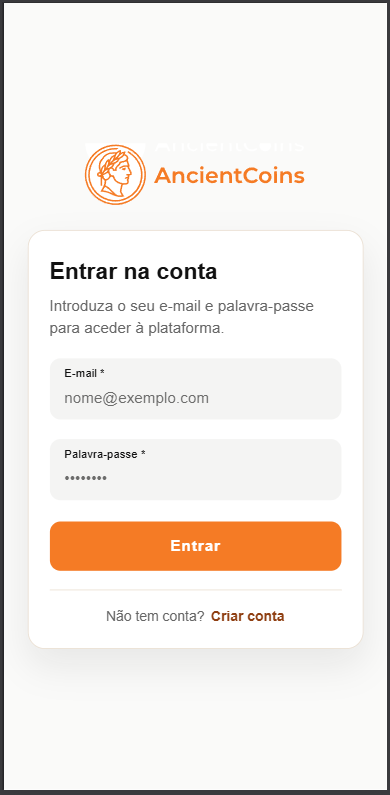
\includegraphics[height=0.43\textheight,keepaspectratio]{01_login.png}\\
\small Login
\end{minipage}
\hfill
\begin{minipage}{0.45\textwidth}
\centering
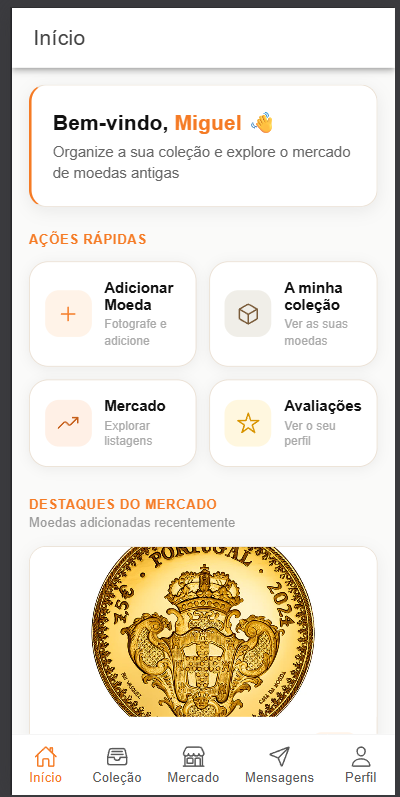
\includegraphics[height=0.43\textheight,keepaspectratio]{02_inicio.png}\\
\small Página inicial
\end{minipage}
\caption{Ecrã de autenticação e página inicial da aplicação AncientCoins.}
\end{figure}

Na área da coleção, o utilizador consegue consultar as moedas registadas, pesquisar por nome ou origem e identificar rapidamente preço, material, condição e estado de venda. O mercado apresenta uma lógica semelhante, mas orientada para exploração, compra e troca de moedas publicadas por outros colecionadores.

\begin{figure}[htbp]
\centering
\begin{minipage}{0.45\textwidth}
\centering
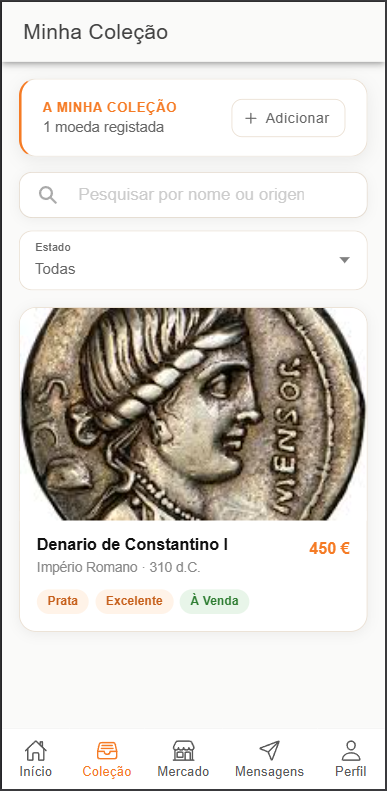
\includegraphics[height=0.43\textheight,keepaspectratio]{03_colecao.png}\\
\small Minha Coleção
\end{minipage}
\hfill
\begin{minipage}{0.45\textwidth}
\centering
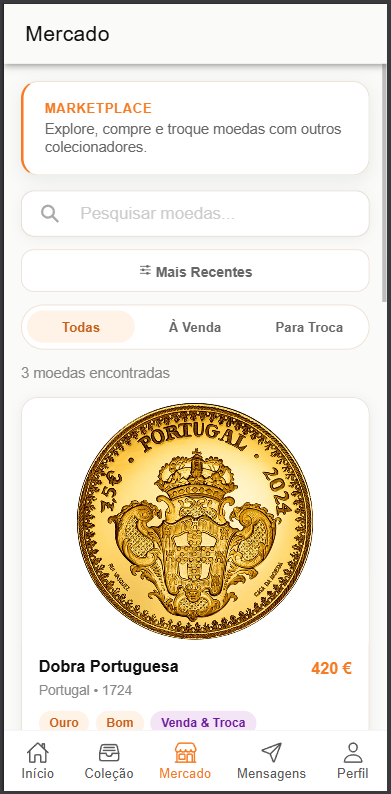
\includegraphics[height=0.43\textheight,keepaspectratio]{04_mercado.png}\\
\small Mercado
\end{minipage}
\caption{Gestão da coleção pessoal e exploração do marketplace.}
\end{figure}

O ecrã de mensagens centraliza as conversas associadas a negociações, mostrando remetente, moeda relacionada, data e pré-visualização da última mensagem. O perfil resume a conta do utilizador, a localização, a avaliação e estatísticas relevantes, como moedas registadas, moedas publicadas e valor em mercado.

\begin{figure}[htbp]
\centering
\begin{minipage}{0.45\textwidth}
\centering
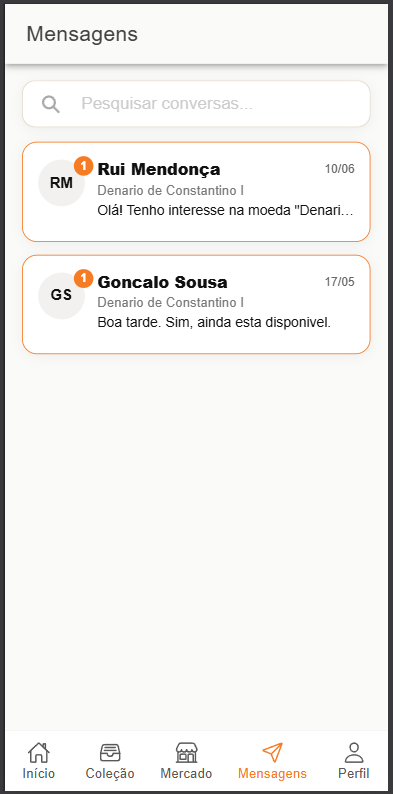
\includegraphics[height=0.43\textheight,keepaspectratio]{05_mensagens.png}\\
\small Mensagens
\end{minipage}
\hfill
\begin{minipage}{0.45\textwidth}
\centering
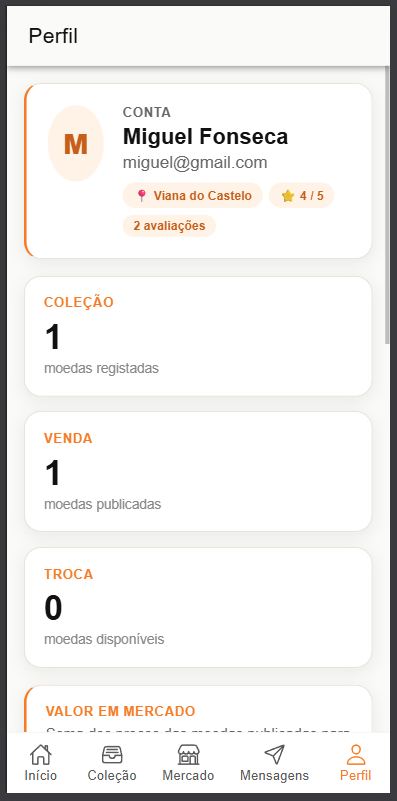
\includegraphics[height=0.43\textheight,keepaspectratio]{06_perfil.png}\\
\small Perfil
\end{minipage}
\caption{Comunicação entre utilizadores e síntese do perfil do colecionador.}
\end{figure}

O formulário de adicionar moeda foi estruturado para suportar a catalogação completa da peça, incluindo nome, origem, ano, material, condição, descrição e imagem. A secção de mercado permite decidir se a moeda fica disponível para venda ou troca, mantendo o mesmo fluxo de criação.

\begin{figure}[htbp]
\centering
\begin{minipage}{0.45\textwidth}
\centering
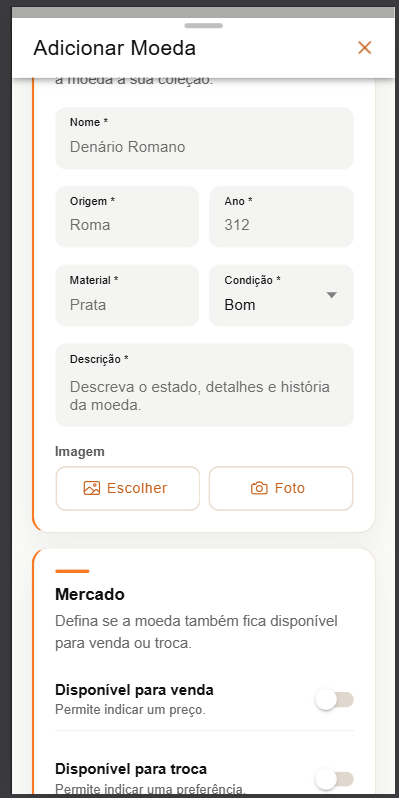
\includegraphics[height=0.43\textheight,keepaspectratio]{07_adicionar_moeda.png}\\
\small Adicionar moeda
\end{minipage}
\hfill
\begin{minipage}{0.45\textwidth}
\centering
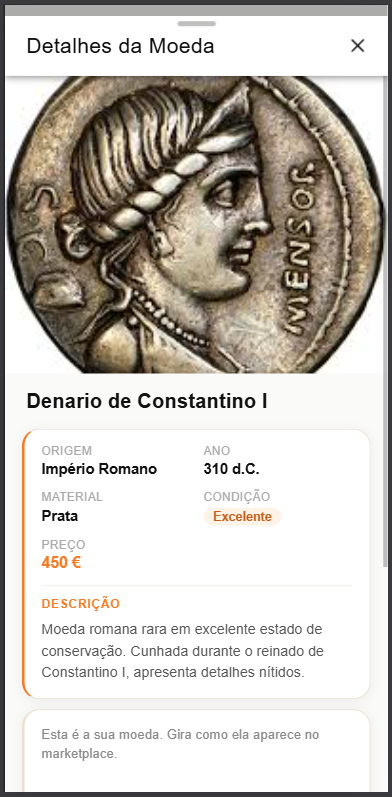
\includegraphics[height=0.43\textheight,keepaspectratio]{08_detalhe_colecao.png}\\
\small Detalhe da moeda na coleção
\end{minipage}
\caption{Formulário de criação e detalhe de uma moeda pertencente ao utilizador.}
\end{figure}

O detalhe de uma moeda no mercado destaca a imagem, os dados principais da peça, a preferência de troca, a descrição e a informação do vendedor. O botão de negociação no rodapé torna a ação principal clara e facilita o contacto entre colecionadores.

\begin{figure}[htbp]
\centering
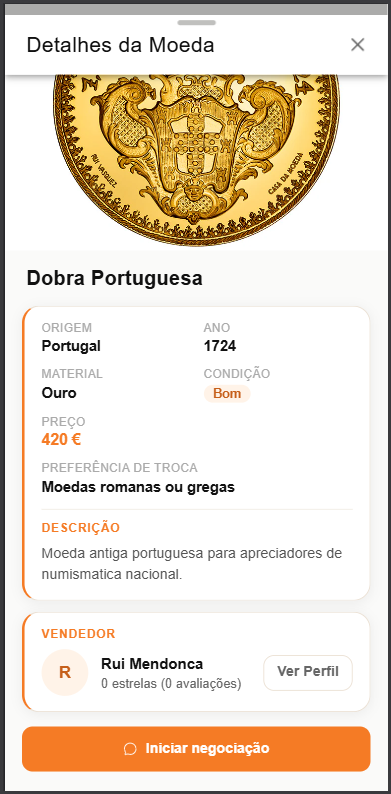
\includegraphics[height=0.56\textheight,keepaspectratio]{09_detalhe_mercado.png}
\caption{Detalhe de uma moeda publicada no mercado, com informação do vendedor e ação de negociação.}
\end{figure}

\subsection{Requisitos Mínimos Implementados}

A versão final da aplicação AncientCoins implementa os requisitos mínimos definidos para o projeto.

\subsubsection{Routing aplicado na navegação da app}

A navegação da aplicação AncientCoins foi implementada recorrendo ao sistema de Routing disponibilizado pelo Angular Router. A estrutura da aplicação encontra-se organizada através de páginas independentes e módulos específicos, permitindo uma navegação fluida entre as diferentes áreas da plataforma.

Foram definidas rotas para autenticação, registo de utilizadores e navegação principal através do sistema de Tabs da aplicação. Esta abordagem permitiu separar claramente as responsabilidades de cada página e facilitar a manutenção do código.

A utilização do Angular Router permitiu ainda implementar mecanismos de proteção de acesso a páginas reservadas para utilizadores autenticados.

Exemplos de rotas implementadas:

\begin{itemize}
\setlength{\itemsep}{0.15em}
\item Login;
\item Registo;
\item Página Inicial;
\item Coleção;
\item Mercado;
\item Mensagens;
\item Perfil;
\item Modais de detalhe das moedas.
\end{itemize}

\subsubsection{Utilização do Angular Router e ActivatedRoute}

Durante o desenvolvimento foram utilizados os serviços Router e ActivatedRoute do Angular para controlar a navegação entre páginas e permitir a passagem de informação entre componentes.

O Router foi utilizado para efetuar redirecionamentos após autenticação, logout e seleção de elementos da aplicação.

O ActivatedRoute foi utilizado para recuperar parâmetros enviados durante a navegação, permitindo apresentar conteúdos específicos associados a moedas, utilizadores e conversas.

Esta abordagem permitiu desacoplar os componentes e reduzir dependências diretas entre páginas.

\subsubsection{Navegação com passagem de parâmetros}

A aplicação suporta a passagem de parâmetros entre páginas e componentes, permitindo transportar informação contextual sem necessidade de recarregamentos completos.

Entre os principais exemplos encontram-se:

\begin{itemize}
\setlength{\itemsep}{0.15em}
\item Identificador da moeda selecionada;
\item Identificador da conversa;
\item Identificador do utilizador;
\item Dados temporários para abertura automática de modais.
\end{itemize}

Esta funcionalidade é utilizada em diversas áreas da aplicação, nomeadamente:

\begin{itemize}
\setlength{\itemsep}{0.15em}
\item Mercado $\rightarrow$ Detalhe da Moeda;
\item Coleção $\rightarrow$ Detalhe da Moeda;
\item Mensagens $\rightarrow$ Conversa;
\item Home $\rightarrow$ Mercado.
\end{itemize}

\subsubsection{Utilização de ícones da framework Ionic}

Foram utilizados diversos ícones disponibilizados pela framework Ionic, nomeadamente para navegação, pesquisa, perfil, mercado, coleção e mensagens.

\subsubsection{Estrutura modular da aplicação}

O projeto encontra-se organizado em:

\begin{itemize}
\setlength{\itemsep}{0.15em}
\item Pages;
\item Components;
\item Services;
\item Models;
\item Assets;
\item Guards.
\end{itemize}

\subsubsection{Manipulação de templates Ionic}

Foram personalizados os templates fornecidos pela framework Ionic para responder às necessidades específicas da aplicação.

\subsubsection{Persistência de informação}

A persistência dos dados da aplicação é assegurada através da integração com a plataforma Supabase.

Os dados dos utilizadores, moedas, mensagens e avaliações são armazenados permanentemente na base de dados remota.

Adicionalmente, são utilizados mecanismos de armazenamento local para manter sessões autenticadas e melhorar a experiência do utilizador entre reinícios da aplicação.

Esta abordagem garante:

\begin{itemize}
\setlength{\itemsep}{0.15em}
\item Persistência dos dados;
\item Sincronização entre dispositivos;
\item Recuperação automática de sessão;
\item Segurança da informação.
\end{itemize}

\subsubsection{Utilização de ficheiros JSON}

Durante as fases iniciais de desenvolvimento foram utilizados ficheiros JSON para simulação de dados e testes dos componentes visuais.

Os ficheiros continham informação relativa a:

\begin{itemize}
\setlength{\itemsep}{0.15em}
\item moedas;
\item utilizadores;
\item mensagens;
\item avaliações.
\end{itemize}

Esta abordagem permitiu validar a interface antes da integração completa com a base de dados Supabase.

Posteriormente os dados mock foram substituídos por informação real proveniente do backend.

\subsubsection{Utilização de Ionic Components}

Foram utilizados diversos componentes nativos da framework:

\begin{itemize}
\setlength{\itemsep}{0.15em}
\item ion-card;
\item ion-modal;
\item ion-searchbar;
\item ion-tabs;
\item ion-toolbar;
\item ion-button;
\item ion-input;
\item ion-content.
\end{itemize}

\subsubsection{Utilização do Capacitor}

A aplicação utiliza Capacitor para permitir o acesso a funcionalidades nativas do dispositivo móvel.

Foram utilizadas funcionalidades como:

\begin{itemize}
\setlength{\itemsep}{0.15em}
\item acesso à câmara para fotografar moedas;
\item seleção de imagens da galeria;
\item geração do splash screen;
\item geração do ícone da aplicação;
\item empacotamento Android.
\end{itemize}

\subsubsection{CSS Custom Properties}

Foram utilizadas CSS Custom Properties para centralizar a configuração visual da aplicação.

Esta abordagem permitiu reutilizar cores, espaçamentos e estilos de forma consistente em todos os componentes.

As principais propriedades definidas incluem:

\begin{itemize}
\setlength{\itemsep}{0.15em}
\item cor primária da marca;
\item cor secundária;
\item cores de fundo;
\item sombras;
\item raios de borda;
\item tipografia.
\end{itemize}

Esta estratégia facilitou a manutenção e evolução do design visual.

\subsubsection{Personalização global de estilos}

Foi desenvolvido um sistema visual consistente baseado em SCSS, utilizando ficheiros globais para garantir uniformidade em toda a aplicação.

Foram definidos estilos comuns para:

\begin{itemize}
\setlength{\itemsep}{0.15em}
\item cartões;
\item formulários;
\item botões;
\item badges;
\item modais;
\item listas;
\item navegação.
\end{itemize}

A personalização global permitiu alinhar toda a interface com a identidade visual definida durante a fase de prototipagem.

\subsubsection{Otimização através de Services}

A lógica de negócio da aplicação foi centralizada em serviços Angular reutilizáveis.

Esta abordagem permitiu:

\begin{itemize}
\setlength{\itemsep}{0.15em}
\item evitar duplicação de código;
\item facilitar manutenção;
\item promover reutilização;
\item separar lógica de negócio da interface.
\end{itemize}

Os principais serviços implementados foram:

\begin{itemize}
\setlength{\itemsep}{0.15em}
\item AuthService;
\item CoinsService;
\item MarketService;
\item MessagesService;
\item ReviewsService;
\item UsersService;
\item SupabaseService.
\end{itemize}

\subsubsection{Definição de cores globais}

Foi criada uma identidade visual própria para a aplicação AncientCoins.

A paleta de cores foi inspirada na temática numismática e nos tons associados a moedas antigas e materiais nobres.

As cores foram definidas globalmente e reutilizadas em toda a aplicação para garantir consistência visual.

Elementos uniformizados:

\begin{itemize}
\setlength{\itemsep}{0.15em}
\item cabeçalhos;
\item cartões;
\item botões;
\item badges;
\item formulários;
\item sistema de navegação.
\end{itemize}

\subsubsection{Comentários no código}

O código-fonte foi documentado com comentários explicativos nos principais componentes, modelos e serviços da aplicação.

Os comentários permitem compreender:

\begin{itemize}
\setlength{\itemsep}{0.15em}
\item responsabilidades de cada componente;
\item funcionamento dos serviços;
\item estrutura dos modelos de dados;
\item algoritmos de validação;
\item integração com o Supabase.
\end{itemize}

A documentação interna contribui para a manutenção futura e facilita a compreensão do projeto por outros programadores.

\subsubsection{Controlo de versões}

Todo o desenvolvimento foi realizado através do Git e GitHub.

Repositório GitHub: \url{https://github.com/goncalojbsousa/ancient-coins}

\subsubsection{Utilização de Inteligência Artificial}

Foi criado um documento específico indicando todas as tarefas realizadas com apoio de IA.

\subsubsection{Diário de Desenvolvimento}

Foi mantido um diário de desenvolvimento individual por cada elemento do grupo, documentando todas as sessões de trabalho realizadas durante o projeto.

\subsection{Requisitos Adicionais}

Além dos requisitos mínimos obrigatórios, foram implementados diversos requisitos adicionais.

\subsubsection{Utilização de Base de Dados}

A aplicação utiliza o Supabase como Backend-as-a-Service (BaaS), responsável pela autenticação, armazenamento e gestão dos dados.

A estrutura da base de dados inclui tabelas para:

\begin{itemize}
\setlength{\itemsep}{0.15em}
\item utilizadores;
\item moedas;
\item mensagens;
\item avaliações.
\end{itemize}

O Supabase assegura persistência, sincronização e acesso seguro à informação.

\subsubsection{Isolamento de Strings}

Grande parte dos textos utilizados na aplicação encontra-se centralizada nos componentes e serviços, permitindo futura internacionalização.

\subsubsection{Consumo de APIs}

A aplicação comunica com o backend Supabase através da biblioteca oficial JavaScript.

Operações realizadas:

\begin{itemize}
\setlength{\itemsep}{0.15em}
\item autenticação;
\item consulta de moedas;
\item inserção de moedas;
\item atualização de perfil;
\item envio de mensagens;
\item obtenção de avaliações.
\end{itemize}

\subsubsection{Ícone e Splash Screen}

Foram personalizados o ícone da aplicação e o splash screen para refletir a identidade visual do projeto AncientCoins.

\subsubsection{Utilização de Fontes}

Foi utilizada uma tipografia moderna e consistente em toda a aplicação, garantindo legibilidade e uniformidade visual.

\subsubsection{Reactive Forms}

Os formulários da aplicação foram desenvolvidos utilizando Reactive Forms do Angular.

Esta abordagem permitiu implementar:

\begin{itemize}
\setlength{\itemsep}{0.15em}
\item validação em tempo real;
\item campos obrigatórios;
\item validação numérica;
\item controlo de estados dos formulários;
\item mensagens de erro personalizadas.
\end{itemize}

Os Reactive Forms foram utilizados principalmente em:

\begin{itemize}
\setlength{\itemsep}{0.15em}
\item Login;
\item Registo;
\item Adicionar Moeda;
\item Editar Perfil.
\end{itemize}

A utilização desta tecnologia contribuiu significativamente para a qualidade dos dados introduzidos pelos utilizadores.

\section{Problemas Encontrados e Soluções Implementadas}

\subsection{Problemas Encontrados}

Durante o desenvolvimento foram identificados vários desafios técnicos e de design, nomeadamente:

\begin{itemize}
\setlength{\itemsep}{0.15em}
\item Integração entre o Ionic Framework e o Supabase, especialmente na gestão de sessões e chamadas assíncronas;
\item Gestão do estado da aplicação entre componentes e páginas;
\item Uniformização visual entre as diferentes páginas da aplicação;
\item Navegação entre componentes em contextos de tabs e modais;
\item Persistência de dados e sincronização com o backend;
\item Gestão do fluxo de mensagens e atribuição de avaliações.
\end{itemize}

\subsection{Soluções Implementadas}

Para ultrapassar os desafios identificados, foram adotadas as seguintes estratégias:

\begin{itemize}
\setlength{\itemsep}{0.15em}
\item Centralização da lógica de negócio em serviços Angular reutilizáveis;
\item Utilização de modelos de dados consistentes e tipados com TypeScript;
\item Reutilização de componentes Angular para garantir uniformidade visual;
\item Uniformização de estilos através de uma folha SCSS partilhada com variáveis globais;
\item Integração completa com as APIs do Supabase para autenticação e acesso a dados;
\item Utilização de Git e GitHub para controlo de versões e colaboração na equipa.
\end{itemize}

\section{Trabalho Desenvolvido pelos Elementos do Grupo}

\subsection{Rui Mendonça - 29738}

\begin{itemize}
\setlength{\itemsep}{0.15em}
\item Desenvolvimento da área de Mercado;
\item Desenvolvimento da área de Perfil;
\item Integração com Supabase;
\item Implementação do sistema de mensagens;
\item Implementação do sistema de avaliações;
\item Uniformização visual da aplicação;
\item Correção de bugs;
\item Produção de documentação técnica.
\end{itemize}

\subsection{Cristiano Fonseca - 29725}

\begin{itemize}
\setlength{\itemsep}{0.15em}
\item Navegação Tabs
\item Login e autenticação
\item Home
\item Coleção
\item Modais de detalhe
\item Adicionar moedas
\item Upload de imagens
\item Sistema de mensagens
\item Avaliações
\item Storage
\item Melhorias de UX/UI
\end{itemize}

\subsection{Gonçalo Sousa - 29726}

\begin{itemize}
\setlength{\itemsep}{0.15em}
\item Estrutura inicial do projeto Ionic/Angular
\item Models
\item Services
\item DatabaseService (fase inicial)
\item AuthService
\item CoinsService
\item MarketService
\item MessagesService
\item Migração para Supabase
\item Supabase Auth
\item Estrutura SQL
\item Models TypeScript
\item Integração Backend/Frontend
\end{itemize}

\section*{Conclusão}
\addcontentsline{toc}{section}{Conclusão}

O projeto AncientCoins permitiu aplicar de forma prática os conhecimentos adquiridos na unidade curricular de Interação Homem-Máquina, desde a análise inicial dos utilizadores até à implementação e avaliação da solução final.

A aplicação desenvolvida apresenta um conjunto de funcionalidades que respondem às necessidades identificadas durante a fase de análise, permitindo aos colecionadores gerir as suas coleções, negociar moedas e interagir com outros utilizadores de forma simples e intuitiva.

Os resultados obtidos demonstram que os objetivos inicialmente definidos foram alcançados, constituindo uma base sólida para futuras evoluções do sistema. A metodologia seguida - centrada no utilizador e assente em iterações de design e avaliação - revelou-se determinante para a qualidade e consistência do produto final.

\section{Referências Bibliográficas}

Nielsen, J. (1994). Usability Engineering. Academic Press.

Ionic Framework Documentation. \url{https://ionicframework.com}

Angular Documentation. \url{https://angular.dev}

Supabase Documentation. \url{https://supabase.com}

Material de apoio disponibilizado na Unidade Curricular de Interação Homem-Máquina.

\end{document}

